\documentclass{article}
\usepackage{graphicx,url}
\usepackage[brazil]{babel}
\usepackage[utf8]{inputenc}
\usepackage{enumerate}
\usepackage{tabularx}
\usepackage{multirow}
\usepackage{amsmath}
\usepackage[table,xcdraw]{xcolor}

\title{Proposta de Pesquisa: \\
Ferramentas para Relatório de Negócio com Suporte à XBRL
}
\author{Vagner Clementino \\
       \url{vagnercs@dcc.ufmg.br}}
\date{Setembro de  2015}


\begin{document}

\maketitle

\section{Introdução}
\label{sec:intro}

O presente documento tem por objetivo descrever uma proposta de
trabalho acadêmico que  consiste na realização de uma Revisão Sistemática da
Literatura sobre o tema \textit{ferramentas para Relatórios de Negócio com suporte à linguagem XBRL}. Uma \textit{Revisão Sistemática da Literatura} - SLR (do inglês Systematic Literature Review) é uma
metodologia científica cujo objetivo é identificar, avaliar e interpretar
\textit{toda} pesquisa \textit{relevante} sobre uma questão de
pesquisa, área ou fenômeno de
interesse\cite{keele2007guidelines,wohlin2012experimentation}. \textit{Relatórios
  de Negócio (Business Report)} é o produto final do  processo de divulgação
pública de dados operacionais e financeiras de uma organização ou
ainda a prestação regular de informações para os gestores dentro
de uma empresa visado apoiá-los no processo de tomada de decisão.
\cite{lymer1999business}. Há uma terceira via da área de  Relatórios de Negócio
está relacionada ao processo de prestação de contas por entes públicos aos
governos nacionais. A XBRL (\textit{eXtensible Relatórios de Negócio
  Language}) é uma linguagem para divulgação e intercâmbio de
informações financeiras baseada em
XML\cite{xbrl_conceitos_aplicacoes}. O padrão vem sendo adotado por
diversas instituições e empresas em todo mundo com o suporte de um
consórcio global\footnote{\url{www.xbrl.org}} com mais de 650 membros
que incentivam a criação de jurisdições locais. Atualmente o consórcio
conta com 24 jurisdições, sendo que em países como  Estados Unidos,
Grã-Bretanha e Austrália, a XBRL já é a linguagem oficial para entrega
de relatórios à órgãos de governo. A Figura \ref{fig:world_map} exibe
os países que estão promovendo a adoção da XBRL. Estes países estão
com a coloração mais escura no mapa-múndi.

\begin{figure}[htb]
\centering
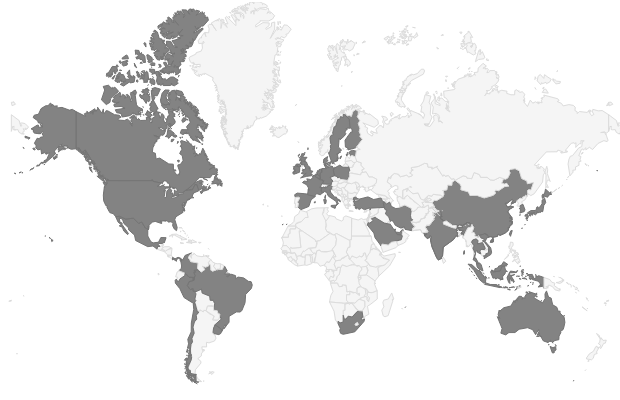
\includegraphics[width=.75\textwidth]{../img/world-map.png}
\caption{O uso da XBRL no mundo}
\label{fig:world_map}
\end{figure}

Nas próximas seções iremos detalhar o estudo proposto
inicialmente discutindo a justificativa do trabalho  e posteriormente
detalhando um estudo prévio realizado conforme as diretrizes propostas
por \cite{kitchenham2009systematic}.
\section{Justificativa}
\label{sec:contexto}

Tendo em vista determinação da Secretaria do Tesouro Nacional, órgão
vinculado ao  Ministério da Fazenda do Brasil, que definiu o XBRL como
padrão para o envio de relatórios de prestação de contas pelos entes
federativos (estados e municípios), surge a necessidade por parte
destes últimos do \textit{desenvolvimento ou aquisição} de sistemas de
informação capazes de criar, processar e enviar informações no formato
XBRL. Como o objetivo de deixar mais claro o contexto no qual esta
necessidade se apresenta analisemos a seguir um cenário em que o
problema se apresenta conforme a narrativa a seguir:
\\
\\
\begin{center}
\fbox{
\begin{minipage}{28em}
Arnaldo é gerente de projeto em uma empresa responsável pelo
desenvolvimento de sistemas para uma prefeitura de médio porte no
estado de Minas Gerais. Ele foi informado pela diretoria da empresa
que devido à mudanças legais, definidas pela Secretaria do Tesouro
Nacional, as prestações de contas da prefeitura para o governo federal
devem ser realizadas em um novo formato denominado XBRL, acrônimo de
eXtensible Business Report Language. Arnaldo sabe que os sistemas
de informação à serviço da prefeitura já são capazes de enviar
relatório aos órgãos fiscalizadores nos formatos CSV (Comma-separated
values) e xls (Microsoft Excel Binary File Format). Após uma análise
do problema, o gerente estabelece dois possíveis caminhos para atender a demanda da prefeitura:

\begin{enumerate}[(i)]
\item Adquirir ferramenta de terceiros com suporte à prestação de contas no formato XBRL;
\item Desenvolver na própria empresa um sistema de informação que possibilite a prestação de conta no formato requirido mas que também possibilite a geração nos formatos já utilizados;
\end{enumerate}

Naturalmente ambas soluções possuem aspectos que podem ser
considerados \textit{positivos e negativos}. Caso a
organização opte por \textit{adquirir} (opção (i)) ela não precisará
enfrentar o risco do baixo conhecimento que existe atualmente na
equipe com relação ao assunto \textit{XBRL}. Todavia, o sistema
comprado de terceiros poderá não atender a todos aos requisitos sendo necessário uma adequação posterior, no qual implicam em um maior custo
para a organização. De outra forma, a criação de um projeto (opção
ii) possui uma maior probabilidade de aderência aos requisitos, em
contrapartida possui os desafios naturais da construção de um sistema
a partir do zero.

A fim de subsidiar a decisão de qual opção a ser tomada, Arnaldo realiza
uma busca na Internet de por comparações entre ferramentas para
Relatórios de Negócio com suporte à XBRL, contudo, os resultados se mostram
incipientes. Ele novamente utiliza uma ferramenta de busca com
objetivo de pesquisar sobre boas práticas e lições apreendidas que
possa ajudar na construção de ferramentas para Relatórios de Negócio e novamente fica decepcionado com os dados retornados. Arnaldo sente-se frustrado por não conseguir referências que o ajude em definir entre a solução (i) e (ii).
%}
\end{minipage}
}
\end{center}

Ao analisarmos o problema descrito no estudo de caso do gerente
Arnaldo, verifica-se que existe a necessidade por parte das
organizações, especialmente as entidades públicas, de referências de
qualidade sobre o assunto de \textit{Ferramentas para Relatórios de
  Negócio com Suporto à XBRL}. Trabalhos com este enfoque
podem \textit{subsidiar a tomada de decisão} por parte dos gestores
públicos. Por exemplo, para aqueles inclinados para a \textit{solução
  (i)} podem utilizar uma  \textit{Revisão Sistemática da
  Literatura} - SLR (do inglês Systematic Literature Review) que
avalie as ferramentas para Relatórios de Negócio que dão suporte ao
XBRL. No caso daqueles voltados para a  \textit{solução (ii)} a
estratégia empírica que melhor daria suporte seria um Pesquisa com Usuários
\textit{Survey} que colete dados de diferentes partes
interessadas (stakeholders) sobre o processo de prestação de contas
das diversas prefeituras do país e avalie as melhores práticas
e lições aprendidas no desenvolvimento e utilização de sistema de
informação para esta finalidade.

Neste contexto, propõe com este trabalho a realização de Revisão
Sistemática da Literatura bem como de uma Pesquisa com Usuário
(Survey). Uma \textbf{Pesquisa com Usuário (Survey)} é um processo de
coleta de informações de ou sobre
\textit{pessoas} para descrever, comparar ou explicar seus
conhecimentos, atitudes e comportamento sobre um determinado
assunto\cite{fink2003survey}. Uma Pesquisa com Usuário geralmente é conduzida em retrospectiva, ou seja, tem como
objetivo avaliar a utilização por um determinado período de uma
ferramenta ou técnica \cite{kitchenham2009systematic}.

\section{Objetivos do Trabalho}
\label{sec:objetivos}

Este trabalho corresponde a dois estudos empíricos tendo como base a \textit{XBRL}. A primeira parte consiste no
desenvolvimento de uma \textit{Revisão Sistemática da Literatura -
  SLR} sobre ferramentas de \textit{Relatórios de Negócio} com suporte ao
padrão XBRL. O público alvo do referido trabalho são pesquisadores,
programadores, gestores que precisam de uma fonte de informação
independente que avalie as soluções existentes no mercado. A partir
dos dados obtidos da \textit{SLR} deve ser possível, por exemplo, propor
novas ferramentas ou mesmo melhorias nas existentes.

A segunda parte do trabalho é a realização de uma Pesquisa com Usuário
tendo como alvo pessoas que participam diretamente do processo de prestação de contas
entre entes federativos. Dentre estas pessoas podemos citar
contadores, desenvolvedores, gestores e etc que poderiam fornecer
detalhes sobre o atual contexto daquele processo. Os dados fornecidos
por estes profissionais pode ajudar no desenvolvimento de
ferramentas que efetivamente atendam as necessidades de seus diversos usuários.

\section{Revisão Sistemática da Literatura}
\label{sec:rsl}

Uma Revisão Sistemática da literatura (SLR), por se tratar de método
científico, deve seguir uma sequência rigorosa de passos a fim de
alcançar os seus objetivos. Algumas diretrizes orientam o processo de desenvolvimento de uma
SLR\cite{keele2007guidelines}. Algumas destas orientações são listadas
a seguir:
\begin{itemize}
  \item especificar uma ou mais sentenças de buscas que serão
    inseridas nas ferramentas de busca com o objetivo de recuperar os
    estudo preliminares que serão utilizados na revisão;
  \item definir um conjunto de \textit{questões de pesquisa} que
    servirão de norte na condução do trabalho;
 \item  desenvolver um protocolo que definirá os procedimentos a serem adotados durante a revisão, ele servirá como um guia para a condução da revisão.
\end{itemize}

Nas próximas subseções detalhamos cada um dos passos descritos anteriormente.

\subsection{Questões de Pesquisa}
\label{subsec:research_question}

As questões de pesquisa conduzem toda a metodologia
de uma revisão sistemática, em especial: o processo de busca deve identificar estudos
primários que abordam as questões de pesquisa; a extração
deve coletar os itens de dados necessários para responder às
perguntas; a análise de dados deve sintetizar as
informações de tal modo que as perguntas posam ser respondidas.

Para o estudo preliminar foram proposta as seguintes questões de pesquisa:
\begin{itemize}
  \item \textbf{$Q1$}: Quais são as ferramentas de Relatórios de Negócio que
    suportam a XBRL?
  \item \textbf{$Q2$}: Quais são os atributos comuns as ferramentas
    que possibilitem a comparação entre elas?
  \item \textbf{$Q3$}: Existem casos reais de utilização da ferramenta
    (Estudos de Casos, Whitepapers e etc)?
  \item \textbf{$Q4$}: Qual setor da economia (governos, medicina, financeiro) a
    possui exemplos de utilização?
\end{itemize}

Conforme exposto as questões de pesquisas determinam as sentenças de
buscam que possibilitam a coleta dos estudos primários. Na próxima
subseção é será apresentado os resultados do estudo preliminar visando
a definição da sentença de busca \textit{(search string)} mais apropriada.

\subsection{Sentenças de Busca}
\label{subsec:setences}

Como a revisão proposta tem como principal objetivo ser uma referência para aqueles interessados em avaliar ferramentas de Relatórios de Negócio com suporte à XBRL, naturalmente sentenças como ``XBRL", ``tools", ``Relatórios de Negócio"\footnote{Inicialmente será utilizado apenas as sentenças na língua inglesa} se mostram como boas candidatas.

A fim de avaliar qual sentença de busca possibilitaria um conjunto de
estudos preliminares com maior relevância para o trabalho, foi
realizada um estudo prévio utilizando a ferramenta de pesquisa Google
Schoolar\footnote{\url{https://scholar.google.com.br/}}. O estudo é
bastante simples, consistindo apenas em registrar o total de artigos
recuperados quando realizado uma pesquisa com uma sentença $S_n$
qualquer. Não foi utilizado qualquer tipo de filtro na busca (como por
exemplo "por data") e os resultados foram classificados por
relevância. Apesar do simplicidade deste estudo ele se mostra como um
bom ponto de partida para definirmos a sentenças de buscam que
futuramente irão possibilitar a recuperação dos estudos preliminares. A tabela \ref{tab:sentencas} exibe as sentenças utilizadas bem como o total de artigos recuperados.


\begin{table}[]
\centering
\resizebox{\textwidth}{!}{%
\begin{tabular}{clc}
\rowcolor[HTML]{EFEFEF}
{\bf Código da Sentença} & \multicolumn{1}{c}{\cellcolor[HTML]{EFEFEF}{\bf Sentença}} & {\bf Total de Artigos}     \\ \hline
\multicolumn{1}{|c|}{$S_1$} & \multicolumn{1}{l|}{“XBRL”}                                & \multicolumn{1}{c|}{15000} \\ \hline
\multicolumn{1}{|c|}{$S_2$} & \multicolumn{1}{l|}{“XBRL tools”}                          & \multicolumn{1}{c|}{3710}  \\ \hline
\multicolumn{1}{|c|}{$S_3$} & \multicolumn{1}{l|}{“XBRL Business Report tools”}          & \multicolumn{1}{c|}{4110}  \\ \hline
\multicolumn{1}{|c|}{$S_4$} & \multicolumn{1}{l|}{“XBRL tools marketing”}                & \multicolumn{1}{c|}{1290}  \\ \hline
\multicolumn{1}{|c|}{$S_5$} & \multicolumn{1}{l|}{“XBRL Business Report software tools”} & \multicolumn{1}{c|}{2970}  \\ \hline
\end{tabular}
}
\caption{Total de artigos por sentença}
\label{tab:sentencas}
\end{table}

Como pode ser observado a sentença $S_1$ é a consulta mais genérica que poderia ser feita sobre no contexto da XBRL, contudo, é retornado um total de $15000$ um valor relativamente pequeno comparado ao total de artigos retornados ao realizar consultas com o termo ``XML' por exemplo\footnote{A consulta por XML retorna aproximadamente $3 \times 10^{6}$ artigos}.

Não obstante a sentença $S_6$ se mostrou satisfatória tanto pelo total
de artigos recuperados bem como pela relevância dos mesmo, auferida
pela inspeção manual de alguns resultados. Visando avaliar o impacto
de restringir o ano de publicação na sentença $S_6$ foi realizada um
novo conjunto de buscas no qual foi utilizado o critério de seleção
``artigos a parte do ano X''.  Os resultados são exibidos na Figura \ref{fig:graph_artigos_ano}{}.

\begin{figure}[htb]
\label{fig:graph_artigos_ano}
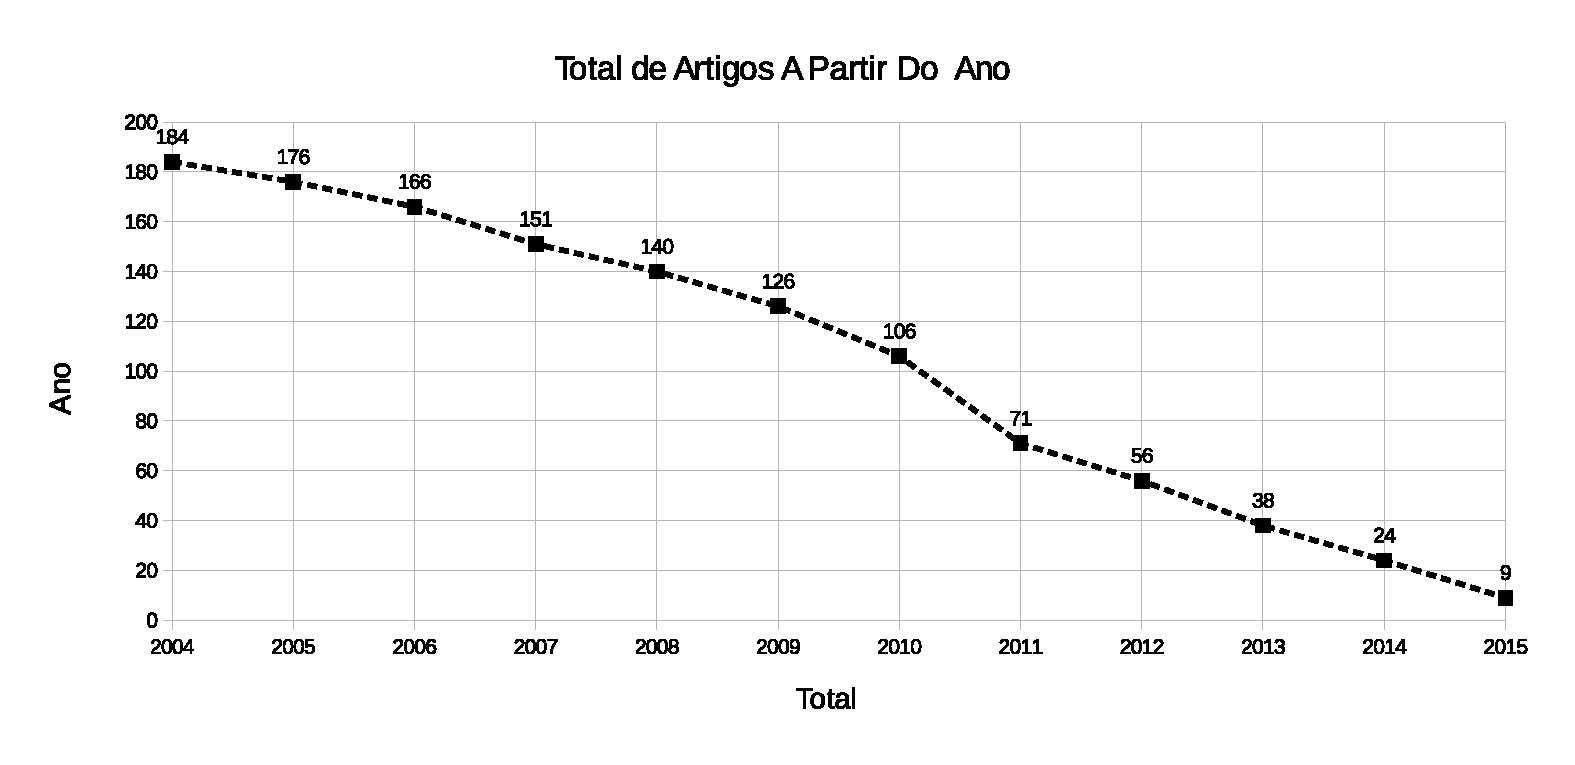
\includegraphics[width=8cm]{../img/graph_01.eps}
\caption{Total de artigo a partir de determinado ano para a sentença $S_6$}
\centering
\end{figure}

A Figura \ref{fig:graph_artigos_ano} mostra conforme esperado a
redução do número de artigos quanto se limita o período de
pesquisa. Em uma análise preliminar pode-se afirmar que a utilização
de artigos publicados a partir de 2012 consegue englobar uma massa de
artigos suficiente para um estudo ponto de partida. Posteriormente,
mediante o Protocolo da Revisão serão definidos critérios para
inclusão e exclusão de ababalho na revisão. Os detalhes destas
diretrizes estão detalhadas na Subseção \ref{subsec:protocol}.



\subsection{Protocolo de Desenvolvimento da Revisão}
\label{subsec:protocol}

Os manuais de diretrizes para Revisões Sistemática em medicina recomenda a
utilização de diversas bases de dados eletrônicas. Neste trabalho utilizou-se
uma lista de indexadores eletrônicos tomando como base o proposto em
\cite{brereton2007lessons,abebe2014trends}, contudo, fazendo algumas alterações. A Tabela \ref{tab:base-dados} exibe
as base de dados eletrônicas utilizadas neste trabalho junto com o total de
trabalhos primários recuperados em cada uma delas

\begin{center}
\begin{tabular}{llllll}
\label{tab:base-dados}
Base de Dados Eletrônica & Nº de Artigos & Percentual\\
\hline
IEEE Xplore  & X & X\\
ScienceDirect  & X & X \\
Springer Link & X & \\
ACM Digital Library & X & X \\
Web of Science & X & X \\
CiteSeer & X & X \\
Wiley Online Library & X & \\
Scopus Elsevier & X &  \\
EL Compendex & X & X \\
Google scholar &  & \\
INSPEC  & X &  \\
\end{tabular}
\end{center}

\section{Survey com Stakeholders}
\label{sec:survey}

Avaliando viabilidade.

\section{Cronograma}
\label{sec:cronograma}


\section{Próximas Etapas}
\label{sec:proximas_etapas}

Aguardando definições.

\medskip

\bibliographystyle{unsrt}%Used BibTeX style is unsrt
\bibliography{../bib/propostaref}

\end{document}
